%%%%%
%%%%% File name  : hw2_report.tex
%%%%% Author     : Yueh-Chou Lee
%%%%% Date       : March 26, 2020
%%%%%
%%
%%%
\documentclass[a4paper,11pt]{article}
\usepackage[top=2cm,bottom=2cm,outer=2cm,inner=2cm]{geometry}
\usepackage[utf8]{inputenc}
\usepackage[T1]{fontenc}
\usepackage{fontspec}
\usepackage{xeCJK}
\usepackage{amsfonts}
\usepackage{amsmath}
\usepackage{graphicx}
\usepackage{subfigure}
\usepackage{setspace}
\usepackage[explicit]{titlesec}
\usepackage{titlesec}
\usepackage{bibentry}
\usepackage[nottoc,numbib]{tocbibind} 
\usepackage{filecontents}
\usepackage{color}
\renewcommand{\baselinestretch}{2}
\setCJKmainfont{標楷體}


\title{Machine Learning Homework 2 Report}
\author{R06221012\hspace{0.2cm}數學所\hspace{0.2cm}李岳洲}
\date{March 26, 2020}

\begin{document}

\maketitle

\begin{enumerate}
	\item \textit{\textbf{請比較實作的 generative model 及 logistic regression 的準確率,何者較佳?請解釋為何有這種情況?}}

	For the training set and the development set, both accuracy scores of logistic regression model are higher than generative model. The reasons should be (1) this dataset is linear classifiable and (2) the number of the dataset is large enough, so that the performance of logistic regression will be better. However, if this dataset is from a probability model, the generative model might be more suitable.\\

	\begin{figure}[htp]
	    \begin{center}
	    	\subfigure[Accuracy]{
	    		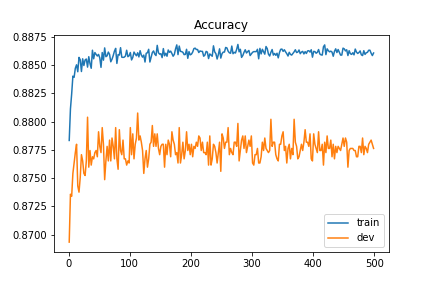
\includegraphics[scale=0.5]{logistic_acc.png}
	    	}
	    	\quad
	    	\subfigure[Loss]{
	    		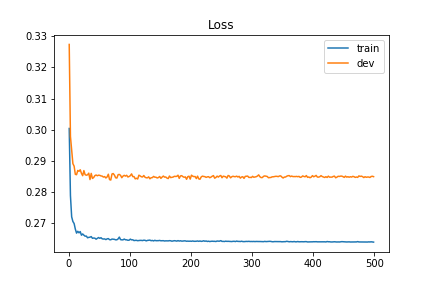
\includegraphics[scale=0.5]{logistic_loss.png}
	    	}
	    	\caption{Logistic model}
	    \end{center}
	\end{figure}

	\begin{table}[htp]
		\begin{center}
			\begin{tabular}{ | c | c | c | c | c |}
			  	\hline
		  		& Training accuracy & Training loss & Development accuracy & Development loss\\[0.5ex] 
		  		\hline \hline
		  		Logistic model & $0.88615$ & $0.26383$ & $0.87836$ & $0.28576$\\[0.2ex]
		  		\hline
		  		Generative model & $0.87470$ & -- & $0.874705$ & -- \\[0.2ex]
		  		\hline
			\end{tabular}
			\caption{Comparison table}
		\end{center}
	\end{table}

	\item \textit{\textbf{請實作 logistic regression 的正規化 (regularization),並討論其對於你的模型準確率的影響。接著嘗試對正規項使用不同的權重 (lambda),並討論其影響。}}

	In the experiments of the regularity adjustment, the accuracy of the development set has increased slightly as the increases in the lambda value, but then decreases. It is deduced that the regularity can reduce the scale of the model parameters to increase the degree of generalization of the model, but as the value of the lambda rises, the original model's underfitting will also cause the accuracy of the train set to decrease, and also cause the accuracy of the development set to decrease.\\


	\begin{table}[htp]
		\begin{center}
			\begin{tabular}{ | c | c | c | c | c | c |}
			  	\hline
		  		Lambda & $0.001$ & $0.01$ & $0.1$ & $1$ & $10$\\[0.5ex] 
		  		\hline \hline
		  		Training accuracy & $0.81699$ & $0.83340$ & $0.86587$ & $0.86690$ & $0.86627$\\[0.2ex]
		  		\hline
		  		Development accuracy & $0.80740$ & $0.82602$ & $0.86325$ & $0.86730$ & $0.86483$\\[0.2ex]
		  		\hline
			\end{tabular}
			\caption{Comparison table (regularization)}
		\end{center}
	\end{table}

	\item \textit{\textbf{請說明你實作的 best model,其訓練方式和準確率為何?}}

	\begin{enumerate}

	\item [\textit{Step 1.}] \textit{Data Preprocessing}

		\begin{enumerate}
			\item [a.] Normalization
		\end{enumerate}

	\item [\textit{Step 2.}] \textit{Features Extraction}

	\textbf{T-test:}

		We collect all 510 features into the $N \times 510$ matrix and then divide into two matrices, the features in the $N_0 \times 510$ matrix are labeled as $0$ and the features in the $N_1 \times 510$ matrix are labeled as $1$. Calculate the $p-$value of each feature, if $p-$value is less than $0.05$, we will select these features to train and predict.

	\item [\textit{Step 3.}] \textit{Train}

	\textbf{Setting:}
			\begin{enumerate}
				\item [a.] Loss function: Cross entropy

				\item [b.] Update of weights: Gradient descent

				\item [c.] Learning rate: 0.0005

				\item [d.] Maximum iteration: 2000

				\item [e.] Early stopping iteration: 20, stop training by judging the validation accuracy.

			\end{enumerate}

	\item [\textit{Step 4.}] \textit{Train again}

	\textbf{Setting:}
			\begin{enumerate}
				\item [a.] Loss function: Cross entropy

				\item [b.] Update of weights: Gradient descent

				\item [c.] Learning rate: 0.000001

				\item [d.] Maximum iteration: 2000

				\item [e.] Early stopping iteration: 100, stop training by judging the validation accuracy.
			\end{enumerate}

		\item [\textit{Result}].

		\begin{table}[htp]
			\begin{center}
				\begin{tabular}{| c | c | c | c | c | }
				  	\hline
			  		& Simple baseline & Simple model & Strong baseline & Best model\\[0.5ex] 
			  		\hline \hline
			  		Accuracy & $0.88617$ & $0.88849$ & $0.89052$ & $0.89131$\\[0.2ex]
			  		\hline
				\end{tabular}
				\caption{Kaggle's public test set accuracy}
			\end{center}
		\end{table}
	\end{enumerate}

	\item \textit{\textbf{請實作輸入特徵標準化 (feature normalization),並比較是否應用此技巧,會對於你的模型有何影響。}}

	Using normalization will be better than using original features. After normalizing features, both the accuracy curve and the loss curve will smoothly increase and decrease, moreover, both curves fast converge to a local minimum and a local maximum. The reasons are (1) each feature has a different scale and (2) different features have very different effects on the loss function of the gradient descent. If we don't use normalization, it will be quite unstable when the loss drops, that's why we need to take more iterations to reach the local minimum.\\

	\begin{figure}[htp]
	    \begin{center}
	    	\subfigure[Training accuracy]{
	    		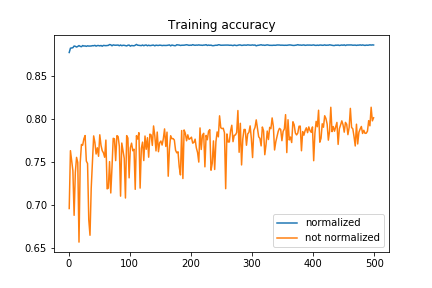
\includegraphics[scale=0.5]{norm_no_norm_train_acc.png}
	    	}
	    	\quad
	    	\subfigure[Training loss]{
	    		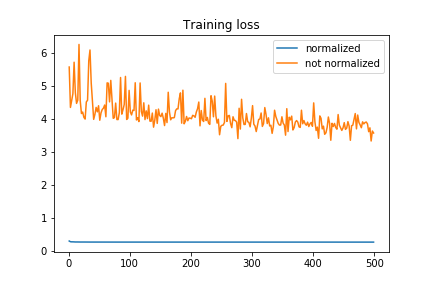
\includegraphics[scale=0.5]{norm_no_norm_train_loss.png}
	    	}
	    	\caption{Training set}
	    \end{center}
	\end{figure}

	\begin{figure}[htp]
	    \begin{center}
	    	\subfigure[Development accuracy]{
	    		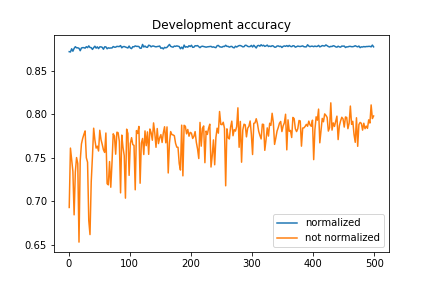
\includegraphics[scale=0.5]{norm_no_norm_dev_acc.png}
	    	}
	    	\quad
	    	\subfigure[Development loss]{
	    		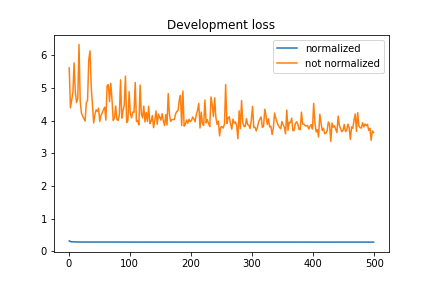
\includegraphics[scale=0.5]{norm_no_norm_dev_loss.png}
	    	}
	    	\caption{Development set}
	    \end{center}
	\end{figure}

	\begin{table}[htp]
		\begin{center}
			\begin{tabular}{ | c | c | c | c | c |}
			  	\hline
		  		& Training accuracy & Development accuracy\\[0.5ex] 
		  		\hline \hline
		  		Normalized & $0.88697$ & $0.88002$ \\[0.2ex]
		  		\hline
		  		No normalized & $0.81914$ & $0.81865$\\[0.2ex]
		  		\hline
			\end{tabular}
			\caption{Comparison table (normalized)}
		\end{center}
	\end{table}

\end{enumerate}
\end{document}